\documentclass{article}
\usepackage{graphicx, color}
\usepackage[a4paper,margin=2cm]{geometry}
\usepackage{url}
\usepackage{subfig}
\usepackage{amsthm}
\newtheorem{definition}{Definition}
\newcommand{\red}[1]{{\color{red}{#1}}}

\begin{document}

	\begin{titlepage}
	
	\newcommand{\HRule}{\rule{\linewidth}{0.5mm}} % Defines a new command for the horizontal lines, change thickness here
	\center % Center everything on the page
	
	%----------------------------------------------------------------------------------------
	%	HEADING SECTIONS
	%----------------------------------------------------------------------------------------
	
	%\includegraphics[width=\linewidth]{uvaENG}\\[2.5cm]
	\textsc{\Large MSc Artificial Intelligence}\\[0.2cm]
	\textsc{\Large Master Thesis}\\[0.5cm] 
	
	%----------------------------------------------------------------------------------------
	%	TITLE SECTION
	%----------------------------------------------------------------------------------------
	
	\HRule \\[0.4cm]
	{ \huge \bfseries \red{Designing custom inconsistent knowledge graphs}}\\[0.4cm] % Title of your document
	\HRule \\[0.5cm]
	
	%----------------------------------------------------------------------------------------
	%	AUTHOR SECTION
	%----------------------------------------------------------------------------------------
	
	by\\[0.2cm]
	\textsc{\Large \red{Thomas de Groot}}\\[0.2cm] %your name
	\red{11320303}\\[1cm]
	
	
	%----------------------------------------------------------------------------------------
	%	DATE SECTION
	%----------------------------------------------------------------------------------------
	
	{\Large \today}\\[1cm] % Date, change the \today to a set date if you want to be precise
	
	\red{36 EC}\\ %
	\red{September 2018 - March 2019}\\[1cm]%
	
	%----------------------------------------------------------------------------------------
	%	COMMITTEE SECTION
	%----------------------------------------------------------------------------------------
	\begin{minipage}[t]{0.4\textwidth}
		\begin{flushleft} \large
			\emph{Supervisor:} \\
			\red{Dr A \textsc{Person} }% Supervisor's Name
		\end{flushleft}
	\end{minipage}
	~
	\begin{minipage}[t]{0.4\textwidth}
		\begin{flushright} \large
			\emph{Assessor:} \\
			\red{Dr A  \textsc{Person}}\\
		\end{flushright}
	\end{minipage}\\[2cm]
	
	%----------------------------------------------------------------------------------------
	%	LOGO SECTION
	%----------------------------------------------------------------------------------------
	
	\framebox{\rule{0pt}{2.5cm}\rule{2.5cm}{0pt}}\\[0.5cm]
	%\includegraphics[width=2.5cm]{figure}\\ % Include a department/university logo - this will require the graphicx package
	\textsc{\large \red{institute name}}\\[1.0cm] % 
	
	%----------------------------------------------------------------------------------------
	
	\vfill % Fill the rest of the page with whitespace
	
\end{titlepage}
\pagenumbering{roman}
% Writing of the report


\newpage
\section*{Acknowledgments}



\newpage
\section*{Abstract}
Based on formal semantics most of the knowledge graphs on the Web of Data can be put to practical use. Unfortunately, a significant number of those graphs is logically inconsistent. This makes reasoning impossible and the knowledge formally useless. While methods exist to deal with contradictions, no systematic way exists to evaluate algorithms for repair or reasoning with inconsistency on large realistic knowledge graphs. Even worse, there is not even a methodology for analysing inconsistency in graphs in the first place. 

While large inconsistent knowledge graphs are available, their size often prohibits their usage for benchmarking. Thus, current research often resorts to synthesised knowledge graphs. In this paper, we present a formal notion of `anti-patterns', generalised basic graph patterns, describing contradictions in knowledge graphs. We present an extraction pipeline that retrieves explanations for contradictions in the LOD-a-lot collection of knowledge graphs and generalise them into what we call `anti-patterns'. We enlist an (almost) complete set of `anti-patterns' found in the LOD-a-lot. Next, we evaluate the set `anti-patterns` on their intrinsic characteristics. Finally, we introduce two usages of those `anti-patterns': first, for knowledge graph analysis and, secondly, for generating systematic samples from knowledge graphs. We showcase the two implementations by analysing a set of knowledge graphs and generating configurable inconsistent subontologies of those of variable size.  

\newpage
\tableofcontents
\newpage
\pagenumbering{arabic}

\section{Introduction}
\textit{Background}. Large open knowledge graphs have increased in size over the last couple of years and are frequently used. Multi-billion statements being the standard instead of the exception. With these enormous knowledge graphs, we try to overcome challenges that have been set out, such as data cleaning, contradiction removal, improving linking between entities, relation linking, or even reasoning over multi-billion statements.

Reasoning with large knowledge graphs is hard due to the size and knowledge graphs are often inconsistent. Even if only one contradiction is stated within the knowledge graph the knowledge graph is inconsistent and any statement is semantically entailed (ex falso quodlibet). While some methods to still be able to reason over inconsistent knowledge graphs, such as paraconsistent reasoning\cite{Kaminski:2015}, most reasoners can not. If even reasoners try to reason with inconsistent knowledge graphs, then the reasoner is only able to return that the graph is inconsistent. With some reasoners being able to find the justifications if the knowledge graph is small enough. 

\textit{Motivation}. Understanding inconsistency and the types of contradictions that occur in large knowledge graphs can give us a better overview of how mistakes are made. This can also help us create techniques to prevent mistakes being made in the first place. While inconsistency still blocks reasoning, giving qualitative and quantitative information about a knowledge graph contributes to a better understanding of large knowledge graphs. Moreover, once inconsistency in knowledge graphs is better understood we can systematically build benchmarks for tools such as reasoning under inconsistency (based on default or defeasible logics) or debugging tools. 

\textit{Method}. In this paper, we developed the formal notion of `anti-patterns', describing contradictions that have been generalised to a minimal set of uninstantiated basic triple patterns that we use to describe a set of contradictions in the knowledge graph. We have designed an extraction pipeline that for an arbitrary, inconsistent knowledge graph can retrieve the `almost' complete set `anti-patterns'. We show this by retrieving such `anti-patterns' from the LOD-a-lot\cite{JavierD:2017}. We also use the set as input for the two implementations we designed. Finally, we designed two implementations, analysis for inconsistent knowledge graphs and a sampling method, that make extensive use of the found `anti-patterns'. 

\textit{Research questions}. The above method informally describes our method. To formalise our we wrote down three research questions that form this paper.

\begin{itemize}
	\item \textbf{RQ1}: Can we describe and define a formal definition for general contradiction patterns, which is persistent throughout all knowledge graphs?
	\item \textbf{RQ2}: How can we retrieve the contradictions that have occurred in the natural knowledge graphs and convert the contradictions into generalised patterns?
	\item \textbf{RQ3}: What main characteristics can describe the general contradiction patterns best, and how can we implement these commonalities to give better qualitative and quantitative information about the general contradiction patterns?
	\item \textbf{RQ4}: Are there methods, or can we design methods that could benefit from using general contradiction patterns in their algorithm? 
	\begin{itemize}
		\item Are we able to improve analytics about contradictions for large knowledge graphs, by giving qualitative and quantitative information about a knowledge graph?
		\item How can we improve sampling, to sample from large inconsistent knowledge graphs with general contradiction patterns, and can we keep we the characteristics invariant from sampling? %Verbeteren
	\end{itemize}
\end{itemize}

\textit{Experiments and implementations}. We have selected two implementations to evaluate our method with real-world examples. Firstly, we have designed a system that can analyse Knowledge graphs. The system retrieves `almost' all the  `anti-patterns' based on contradictions in the LOD-a-lot, and calculates the number of times the `anti-patterns' occur in the knowledge graph. Then, the system return a detailed report of characteristics of knowledge graph.
Secondly, we show the implementation that samples knowledge graphs and then generates subgraphs of the original knowledge graph with a user-specified sample-size and the number of contradictions. 

\textit{Findings}. We have tested our pipeline by extracting an `almost' complete set of `anti-patterns' from the LOD-a-lot\cite{JavierD:2017}, which we made available >>LINK<<. We developed a set of characteristics that can be used to describe `anti-patterns' more consisely. 
We show that there is a or no correlation between the size of the `anti-pattern' and the amount of different `anti-patterns'. 
We tested two implementations by processing a set large knowledge graphs, DBpedia\cite{DBpedia}, and YAGO\cite{YAGO}.
We found that the `anti-patterns' give us a more detailed explanation to about the contradictions in an inconsistent knowledge graph. 
We show how the characteristics change between the datasets with different contradictions occur in different knowledge graphs. We also show that the  distribution of `anti-patterns' remains equal in all samples knowledge graphs. 
Secondly, we show that the sampled knowledge graphs match the set characteristics given by the user, and also match the characteristics of the original knowledge graph.

\textit{Contributions}. We give a definition of `anti-patterns' with respect to inconsistent knowledge graphs. We design an extraction pipeline that can extract `anti-patterns' from any arbitrary knowledge graph. Finally, we show that `anti-patterns' can be used to analyse inconsistent knowledge graphs and to systematically sample inconsistent knowledge graph.

\textit{Structure}. The second and third chapter explain the work that this paper is based on, as well as give some background to the reader about the definitions that we use in this work. In the method, we explain more in detail how the method of `anti-pattern' retrieval works. Section 6  showcases the possible applications that make extensive use from the `anti-pattern' that we retrieved in the method. In section 7 we show the experiments that test our hypotheses, we set in the introduction, and analyse the results. We conclude with a conclusion, with an extension of future work.

\newpage
\section{Related Work}
Justifications are first introduced by Horridge et al. in their paper explaining inconsistent OWL ontologies \cite{Horridge:2009}. In this paper the writers describe the framework used to retrieve the justifications from inconsistent knowledge graphs as minimal subsets of the graphs preserving the inconsistency. This forms an integral part of our algorithm. In the paper, they also explain why it is often time-consuming to retrieve all justifications for ontologies. In the paper by T\"{o}pper et al. \cite{Topper:2012} they, propose a solution to identify contradictions in DBpedia, with handcrafted `anti-patterns'. With the extraction of `anti-patterns' from the Lod-a-lot we have a generalised approach that works on any knowledge graph. \\
Paulheim \cite{HeikoP:2016} showcases the need for a standardised evaluation method. In the survey, they show that researchers sometimes choose different knowledge graph(s) according to their needs, this makes it harder to compare different algorithms. Removing this discrepancy would benefit all of us.\\ 
F\'arber et al. \cite{MichaelF:2017} give an in-depth comparison of several large knowledge graphs, and demonstrates that knowledge graphs hold different metrics. The paper by F\"arber et al. \cite{MichaelF:2017} is expanded upon by Debattista et al. in \cite{Debattista:2018}, in which they analysed 130 datasets from the Linked Open Data Cloud using 27 Linked Data quality metrics. Both papers show that each graph has a different underlying structure and in theory, this even can result in different behaviour of algorithms.

\subsection{Sampling}
In the paper by Jure Leskovec and Christos Faloutsos \cite{Leskovec:2006} several sampling techniques are proposed and compared, and with it they show that even naive sampling such as random walks and 'forest fire' show accurate results, even sampling to 15\% of the original size. 
% \cite{Jin:2011} Albatross sampling, shows a sampling technique designed for loosely connected or disconnected networks, especially for social networks, while
% This technique could be useful for sampling graph networks, as the algorithm gives an even more accurate sample, but due to an extra constraint we've put on with the justifications, this sampling technique could not be applied.
% \cite{Kurant:2011} Towards Unbiased BFS Sampling, In this paper the Kurant et al. are explaining the bias that forms when implementing breath first sampling.
% While this paper has no direct effect on the implementation the information described in the paper is useful to explain why our samples have some discrepancies when it comes to the differences in indegree and outdegree. 
Finally Rietveld et al.\cite{Rietveld:2014} shows that sampling for targeted use, in their case SPARQL coverage is possible, this shows that sampling a knowledge base, for targeted cases can generally be relevant for multiple reasons.

\newpage
\section{Background}
In this section, we provide a set of basic notions that are used throughout the paper, and have already been defined in previous papers.\\

\textit{Basic Triple Pattern}. Basic triple patterns(BTP) are the building blocks of knowledge graphs, with each basic triple pattern consisting out three elements.
These three elements are $<$Subject$>$, $<$Predicate$>$, and $<$Object$>$. All three elements hold different entities. The Subject can be defined as a URI, a blank node or it can be interpreted as a variable. The Predicate represents the relation between the Subject and the Object and is defined as a URI or if unknown as a variable. Finally, the Object is the second resource; this can be a URI, blank node, a literal, or a final variable. A BTP can be instantiated, meaning no element of the triple pattern has a variable, or uninstantiated, an element or multiple elements of the BTP have been replaced with a variable. With an uninstantiated BTP, we can ask a question to the knowledge graph and retrieve instantiated BTPs back. Alternatively, we can check with an instantiated BTP if it exists in the knowledge graph.

\textit{Basic Graph Pattern}. A basic graph pattern (BGP) is a set of basic triple patterns and forms the basis of query matching. The basic graph pattern
can consist out of BTPs that are connected, either through $<$Subject$>$ and $<$Subject$>$, $<$Subject$>$ and $<$Object$>$, or $<$Object$>$ and $<$Object$>$.
Alternatively, the BGP consists out of disconnected BTPs. Same as the BTP a BGP can be instantiated, without variables, or uninstantiated, thus parts of the BGP have been replaced with variables. With basic graph patterns, we can ask more informed questions to the knowledge graph, or find if a BGP exists in the knowledge graph.

\textit{Justification}. A Justification\cite{Horridge:2009} is a set of axioms that acts as an explanation for an entailment.
Formally, a justification is a minimal subset of the original axioms which are sufficient to prove the entailed formula. In this paper we interpret a justification as an explanation of contradiction. Given that our knowledge graphs are sets of triples, our justification are instantiated BPGs and are always minimal set of axioms for a single contradiction. 

Before we go deeper into the problem Approach and the method used it is necessary to first understand a set of key concepts that will be used in the coming chapters, although a general knowledge of mathematics is needed. We will also show where the initial data comes from.

\subsection{Knowledge}
Knowledge graphs are a "graphical" representation of a set of statements with information, the knowledge base. This information can be anything about everything. The data is stored in triple format. These are statements that consist out of a $<$Subject$>$, $<$Predicate$>$, $<$Object$>$. Where the Subject and Object are vertices in the graph and the Predicate is the edge between the subject and the object. Both the vertices and the edges have different properties, related to each other. Even though the size of the graph can change according to the amount of triples it has, the graph is most of the time connected. But this is not necessarily so. \\

\textbf{Definition 1} (Knowledge graph) :\\

To give more structure to the graphs we need a framework that can help to solidify the relations between vertices. This is done with RDS, RDF(s) and OWL.\\
RDF \cite{rdfPrimer:2014} stands for \textbf{r}esource \textbf{d}escription \textbf{f}ramework and is a method of storing data in triple format. These statements, consisting out of the $<$Subject$>$, $<$Predicate$>$, $<$Object$>$. can hold different types. The subject can be defined as a URI or a blank node. The predicate represents the relation between the Subject and the Object, and is always defined as a URI. finally the object is the second resource, this can be a URI, blank node or a literal.
RDF is designed to exchange information between processes and applications without the intervention of humans. The goal was to build a framework that is designed link resources without having to add in expensive parsers to convert the information to the correct format every time a new process is added which wants to use the information.

Extending to this is RDFS, this the RDF schema, with this schema we can allow to define ontologies within RDF. It can be used to give structure to the RDF
RDF(s) and OWL are ontologies from the semantic web community. But they are special in the sense that these languages can be used to reason with. thus making it possible to infer new facts from the knowledge of other triples.

Finally OWL \cite{OWLPrimer:2012}, the Web Ontology Language, designed to represent the language tha can describe things and set of things well with regards to relations. But not only that, in OWL it is also possible to reason with that knowledge and make implicit knowledge explicit, for example reason that a subClassOf(Car, Audi) and subClassOf(Audi, A1 Sportsback). This makes it possible to reason that subClassOf(Car, A1 Sportsback) is also a type of relation that exists. The second type of reasoning that is possible now is inconsistency reasoning. A main part of this paper.

Inconsistencies are mistakes in the knowledge graph. It is possible to have data that contradicts other data. An example is a >>><<< . In this example the error is in that two different parts of the data contradict each other. While this can be true in real life data and happen her the real world. Knowledge bases have a hard time understanding inconsistencies and the moment a inconsistency in the data is found it is no longer possible to reason over the data as this means that we can no longer assume that any part of the data is "correct", while it may perfectly be that case.\\

\textbf{Definition 2} (Inconsistency) :\\

Finally we need a language that helps us extract information or patterns from the knowledge graph. This we do with SPARQL.
SPARQL is a query language, The technique behind SPARQL is to query and find patterns in the graph and tries to match these patterns to the pattern in query. If a hit is found it can be seen as a hit to the match the complete graph pattern of the query. The advantage of SPARQL to others for finding these patterns is that SPARQL is optimized fro the linked data community.  \cite{SPARQLPrimer:2013}

\subsection{Reasoner}
What is a reasoner?

What types of reasoners are there?

Why do we need to use a reasoner?


\subsection{Data}
To provide a good overview about natural occurring data on the web the largest possible dataset full with linked data would be the best starting point. It would not only help with finding naturally occurring errors, but would also help solve any scaling issues that could have occurred with by first experimenting on smaller datasets. The data we are talking about is of course the LOD-a-lot.

\subsubsection{LOD-a-lot}
The LOD-a-lot \cite{JavierD:2017} is one of the largest open source linked knowledge graphs that is readily available. The data is stored in a HDT. Where an HDT is a (Header, Dictionary, Triples) File. In this way the data is structured in a compact manner with a binary serialization format for RDF. Which has the advantage that querying large files is fast due to optimizations done which have been tailored on reading large data set \cite{JavierD:2013}.

To explain further what the data holds we need to first understand what linked data exactly is, specifically linked open data. Linked Open data is the notion of data that is published on the web and conforms to the five stars given to the linked open data. \cite{ChristianB:2009}\\
 - The data is available on the web.\\
 - URIs are given to identify things in the data.\\
 - The URI are given HTTP, such that these can be located and found (dereferencing).\\
 - The data that is returned when found is used with open standards such as RDF.\\
 - the data is linked, it refers to other data that has the same linked open data qualities.\\
 
\newpage
\section{Problem formalization}
\subsection{Formal definition of an `anti-pattern'}
Justifications describe a single contradiction, with each justification being an instantiated BGP. Due to the instantiation, the justification can only describe one contradiction. Anti-patterns are generalisations over justifications as uninstantiated patterns, that match  multiple inconsistent justifications in the knowledge graph. 
%We denote a formal definition of an \textit{`Anti-pattern'}:\\

\begin{definition} 
	An \textit{`Anti-pattern'} \textit{of a knowledge graph G is a minimal set of uninstantiated Basic Triple Patterns that match a justification of an inconsistent subgraph of G.}
\end{definition}

The conversion of a justification(instantiated BPG) to an `Anti pattern' in figure (uninstantiated BPG) is shown in figure  \ref{fig:JustificationtoGeneral}.

\subsection{Problem Description}
At the moment most large knowledge graph have contradictions, but with reasoners only being able to reason on smaller knowledge graphs, we do not know much about the composition of the contradictions in the knowledge graphs. Understanding how the contradictions have formed, or where the contradictions occur, is crucial information when we want to develop better tools that can handle larger knowledge graphs. The second problem is that, while implementing solutions on a large scale is preferable, testing and benchmarking on smaller knowledge graphs that match existing knowledge graphs would be more accurate. As natural knowledge graphs and that have known properties and contradictions instead of synthesised knowledge graphs is preferable. \\

To solve the issues, we split it into three parts. The first part is to locate the contradictions within the knowledge graph. Only contradictions that are known can be treated as such, as sampling later in the pipeline can only work with contradictions that are known beforehand to sample accordingly.
The second part of the problem is the knowledge graph analysis. Analysing the graph gives useful statistics about the knowledge graph, and helps us understand the knowledge graph also with respect to the found inconsistencies in the first part.\\
The final part of the problem is the sampling of the knowledge graph. Is it even possible to sample from the original knowledge base and keep the characteristics we measured in the second part of the problem on the same level as the original large knowledge graph? Moreover, can we make sure that the sampled graph still holds the number of inconsistencies we want the graph to have? We examine this by experimenting with a set of large knowledge graphs and test if we have replicated the original knowledge graph in a smaller variant, as well as a measure if the number of inconsistencies matches the number of inconsistencies we have set.

\newpage
\section{Method}
\begin{figure}[!t]
	\centering
	\makebox[\textwidth][c]{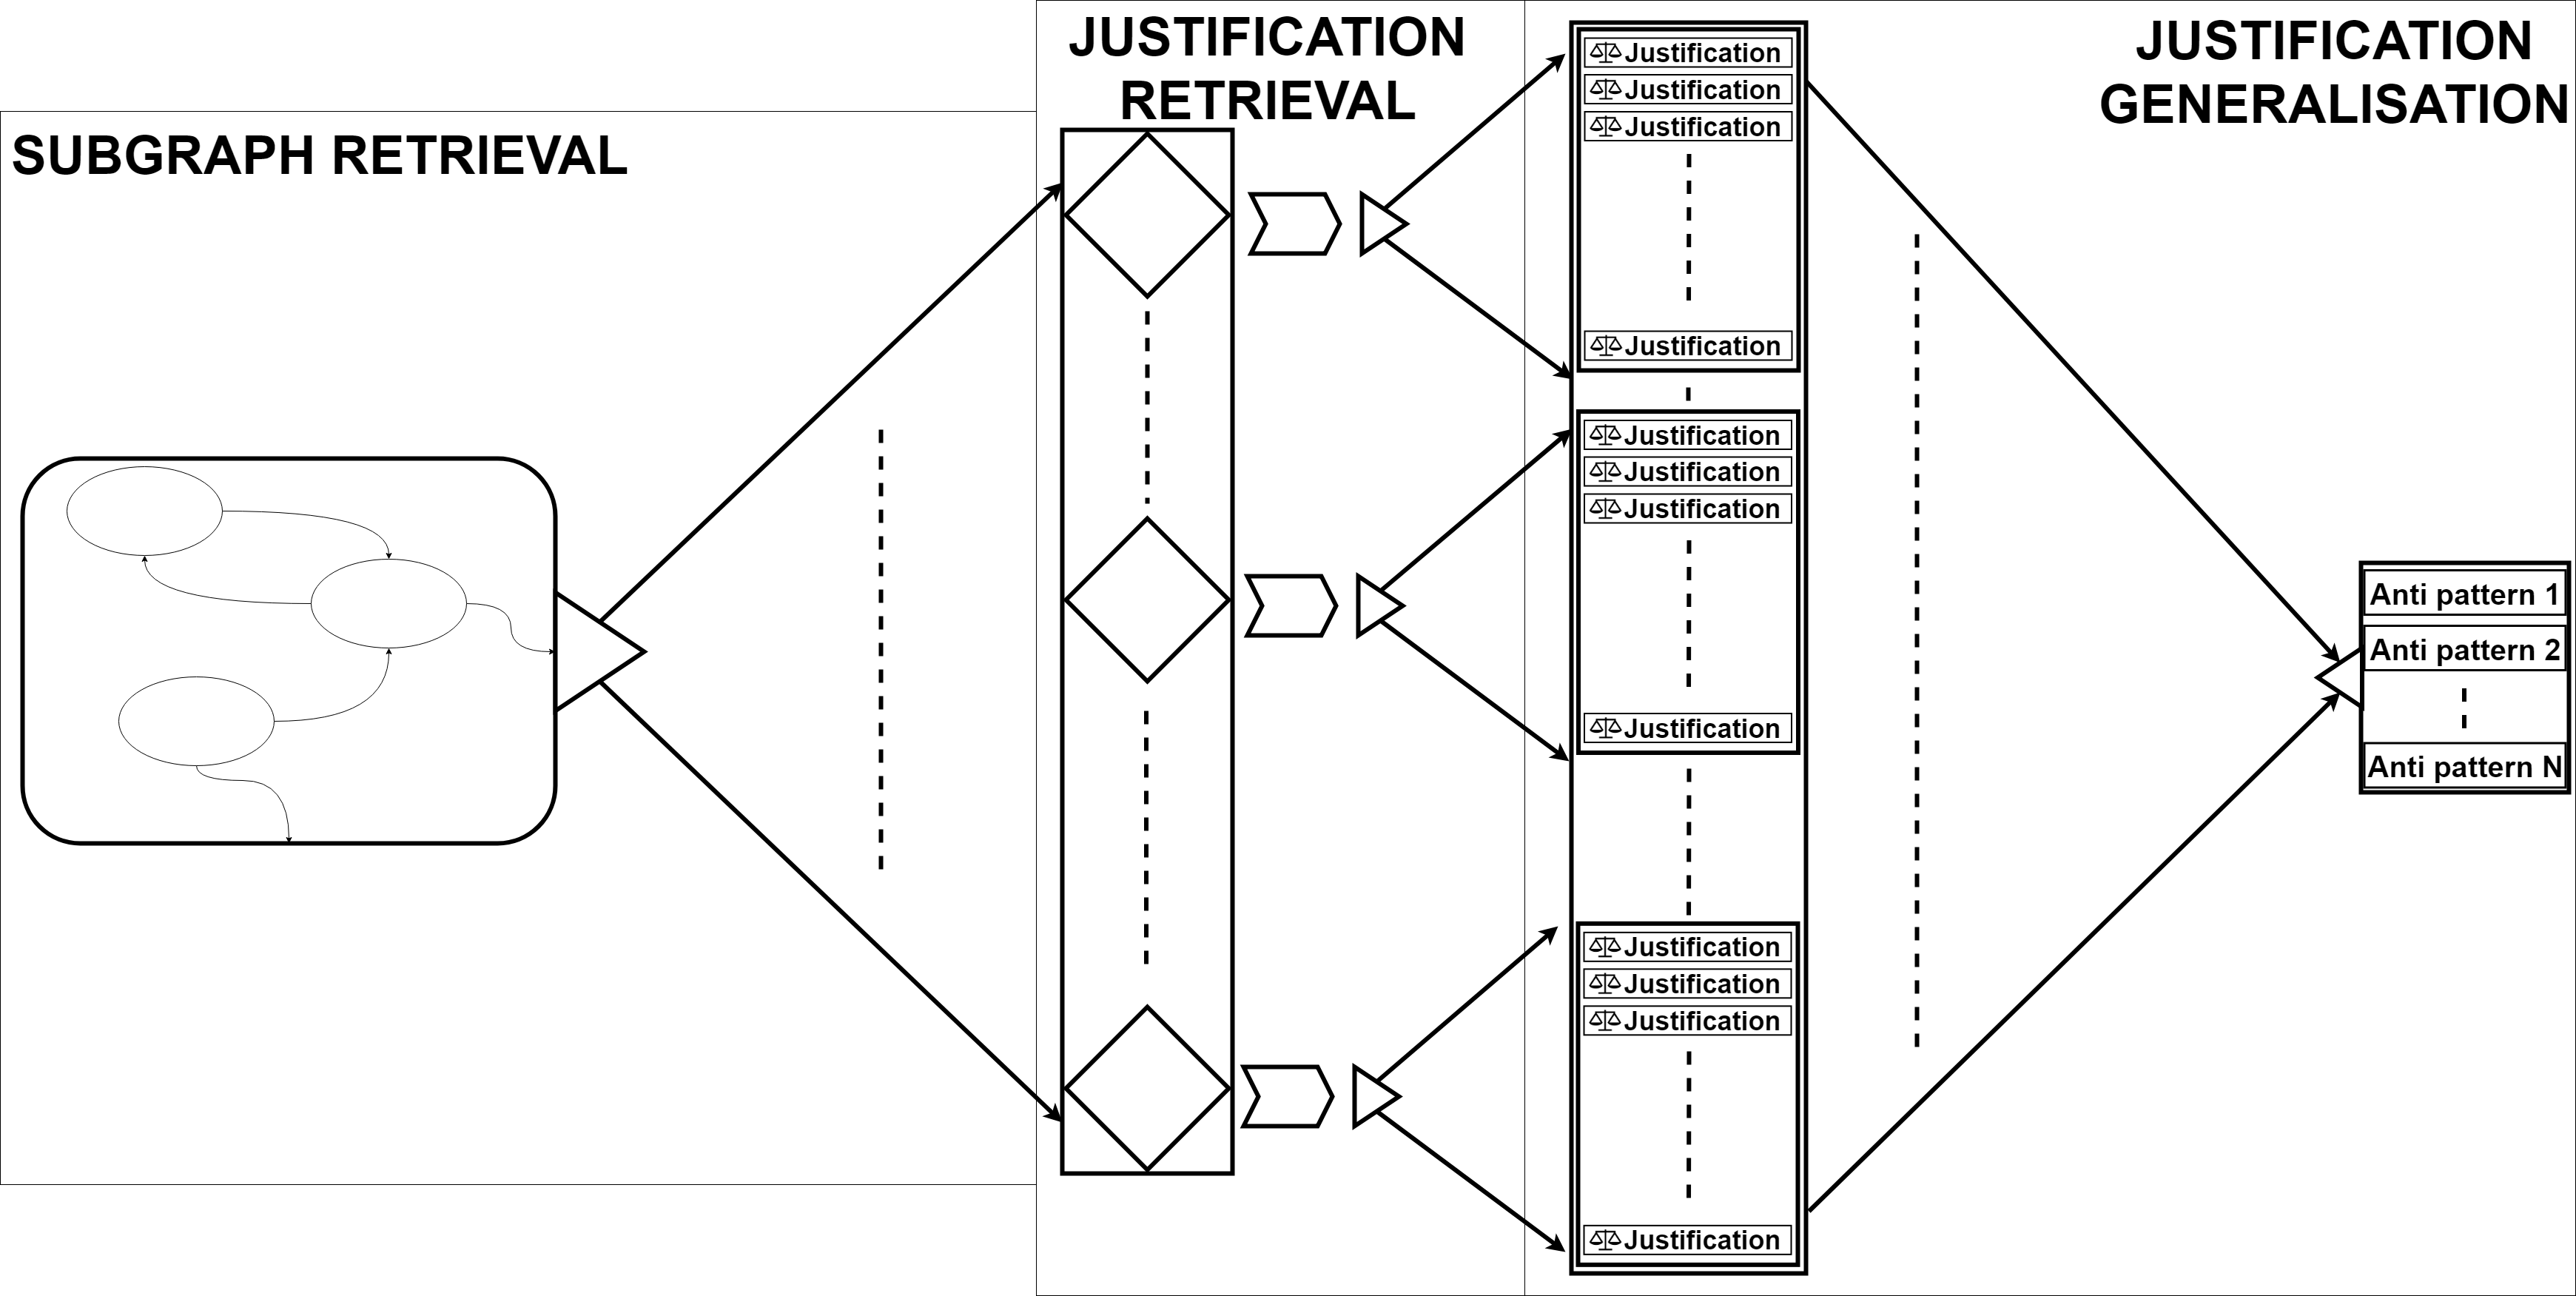
\includegraphics[width=0.8\textwidth]{images/SimplifiedPipelineMissingPart.png}}%
	\caption{A schematic diagram that shows the pipeline used to extract subgraphs, find justifications and their `anti-patterns'. Finally 
		we use the information that we retrieved, to analyse and sample the Knowledge graph.}
	\label{fig:simplePipeline}
\end{figure}
Our extraction method consists of three aspects: Firstly, we retrieve smaller subgraphs from the knowledge graph from which we want the contradictions. Secondly, from each subgraph, we check if the graph is inconsistent and retrieve the justifications. Finally, with the justifications, we create the `anti-patterns'. The entire pipeline is shown in figure \ref{fig:simplePipeline}.\\
Our pipeline is designed to find `almost' all the `anti-patterns' in any knowledge graph. We implemented techniques to find these smaller inconsistent subgraphs with OWLAPI\cite{Horridge:2011} and Openllet\cite{Openllet:2019} which based on work of Pellet\cite{Pellet:2007}.\\

\subsection{Subgraph retrieval}
\begin{figure}[!t]
	\subfloat[A diagram that shows the retrieval and splitting of subgraphs from the knowledge graph.\label{fig:subgraphRetrieval}]{%
		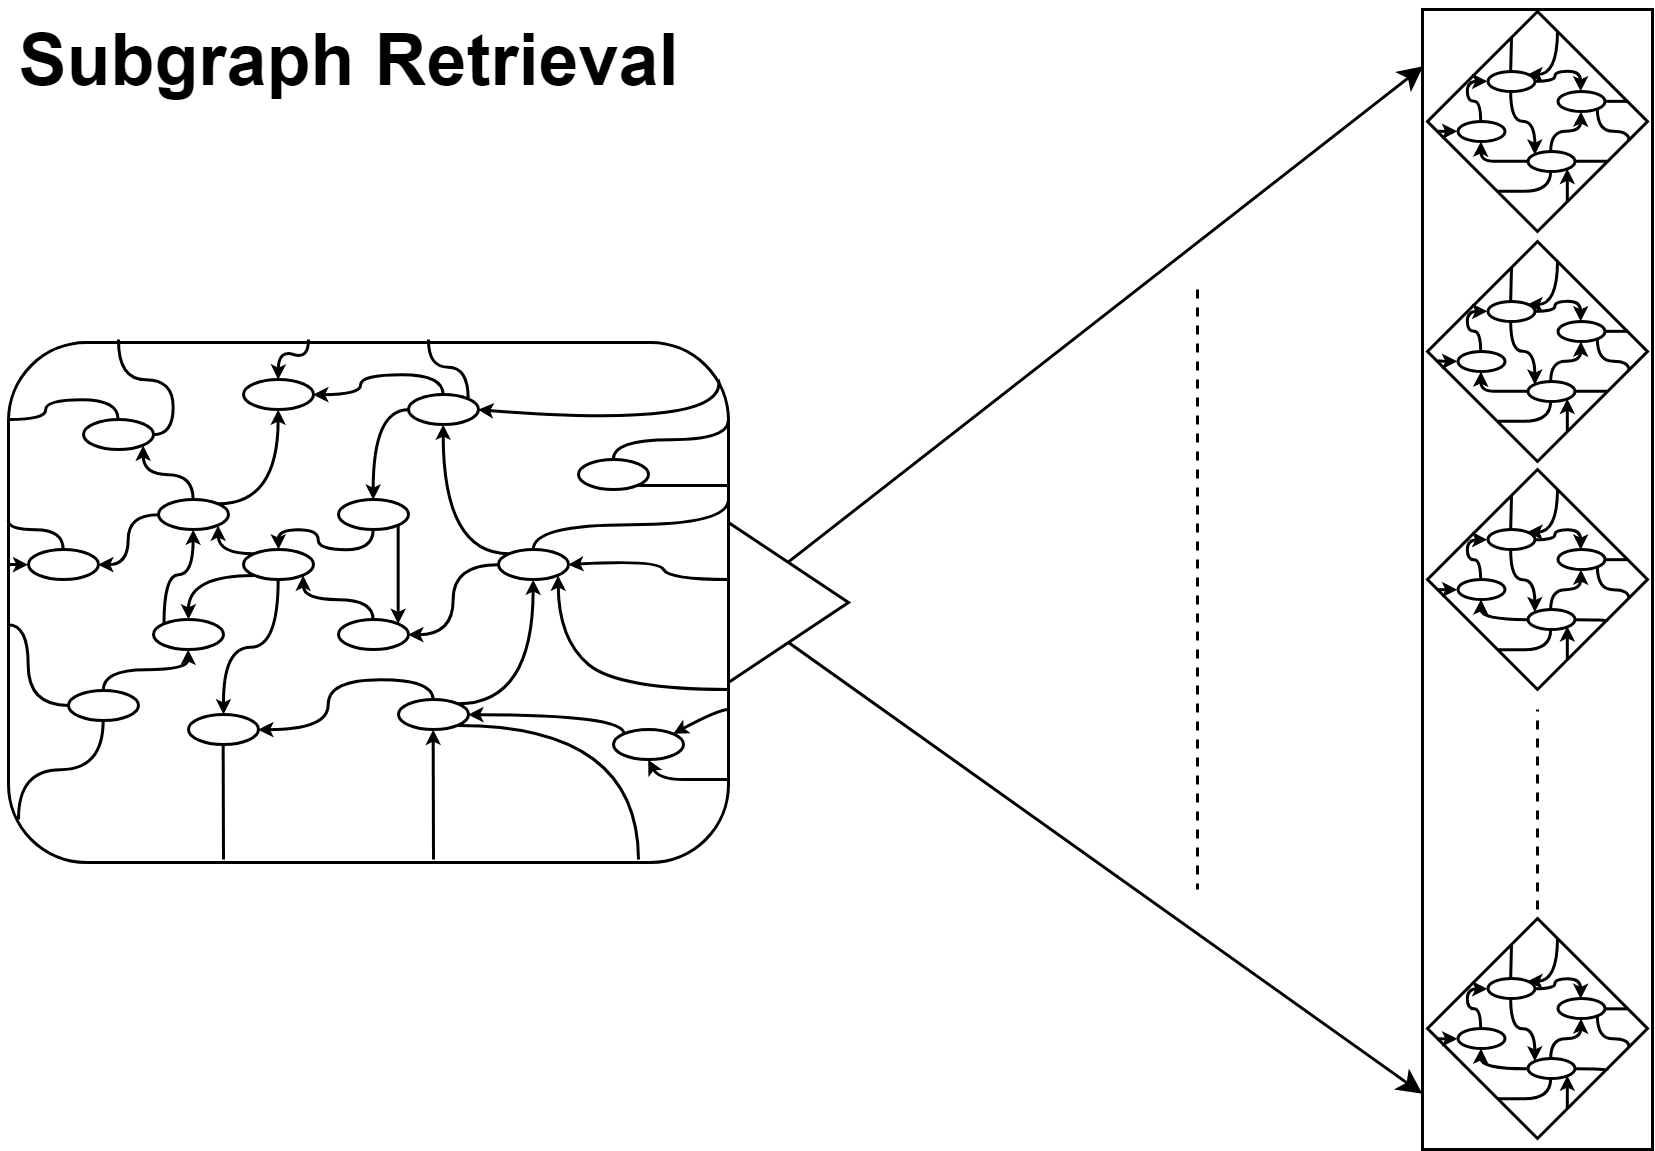
\includegraphics[width=0.45\textwidth]{images/SubgraphRetrieval.png}
	}
	\hfill
	\subfloat[A diagram that shows the retrieval of justifications from a single subgraph.\label{fig:JustificationRetrieval}]{%
		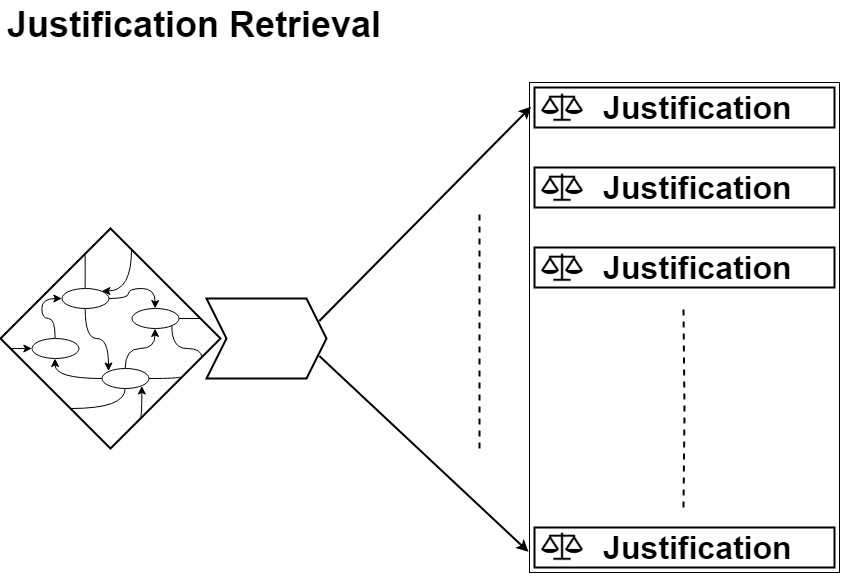
\includegraphics[width=0.45\textwidth]{images/JustificationRetrieval.png}
	}
	\caption{zoomed in diagrams of the first part of the pipeline}
	\label{fig:PipelinePart12}
\end{figure}
Due to the large size of most knowledge graphs, running a justification retrieval algorithm over the complete knowledge graph, to retrieve all contradictions would be impractical. To speed up this process, we decided to split the knowledge graph into smaller chunks to reduce the time the justification retrieval algorithm needs to find all justifications in the smaller subgraphs. Figure \ref{fig:subgraphRetrieval} shows the process of splitting the knowledge graph into smaller subgraphs.
Each subgraph is generated by extending the root node. The root node is retrieved by taking a triple from the complete graph and taking the node that is in the subject position as the starting point. The graph is expanded by finding all the triples that have the root node as the subject, and we add these triples to the subgraph. Next, all the nodes that were in the object position are now used as expansion nodes, so now for each object, we now find all the triples that match where the object is put in the subject position. We keep expanding the graph until it can not expand any further or the maximum amount of triples of 5000 triples is reached. The value of 5000 triples is chosen because it is large enough to hold almost all justification patterns but small enough that it does not take long to retrieve all justifications.\\
While this method to sample subgraphs from the knowledge graph does not guarantee completeness in terms of finding all the contradictions that can occur, but we show that this method finds the `almost' all occurring contradictions, with the help of redundancy, without occurring too many time-consuming calculations. 

\subsection{Justification retrieval}
With the knowledge graph split into smaller chunks, we can now move on the next step in the extraction pipeline, as shown in figure \ref{fig:JustificationRetrieval}.
With the newly formed subgraphs, we start with the check if the graph is consistent or inconsistent. If the graph is consistent, we can skip this graph, as the amount of contradictions is zero.\\ 
If the graph is inconsistent, then we find the reason or reasons why, a graph can be inconsistent due to a single contradiction, or it can have multiple contradictions. 
To find all the contradictions we use the justifications algorithm in the Openllet reasoner. The justifications algorithm walks through the graph and finds the minimal justification for each contradiction. The algorithm continues to search for justifications until no more justification can be found in the graph. This is done for each subgraph, and all the justifications are then pushed through the extraction pipeline to the next stage.\\

\subsection{Justification generalization to `anti-patterns'}
While all justifications are different as each justification is a set of instantiated BTP, the underlying uninstantiated BGP does not have to be. The underlying BGP forms the basis of the `anti-patterns'. The `anti-patterns' describe a set of contradictions, that has been found in the inconsistent knowledge graph. The `anti-patterns' can be used to locate inconsistencies in other knowledge graphs as well. In Figure \ref{fig:PatternGeneralizing} we show the last part of the pipeline, the conversion of all justifications to a set of `anti-patterns'.

\begin{figure}[!t]
	\subfloat[A schematic diagram showcasing how the justifications are transformed into Generalized inconsistency patterns.\label{fig:PatternGeneralizing}]{%
		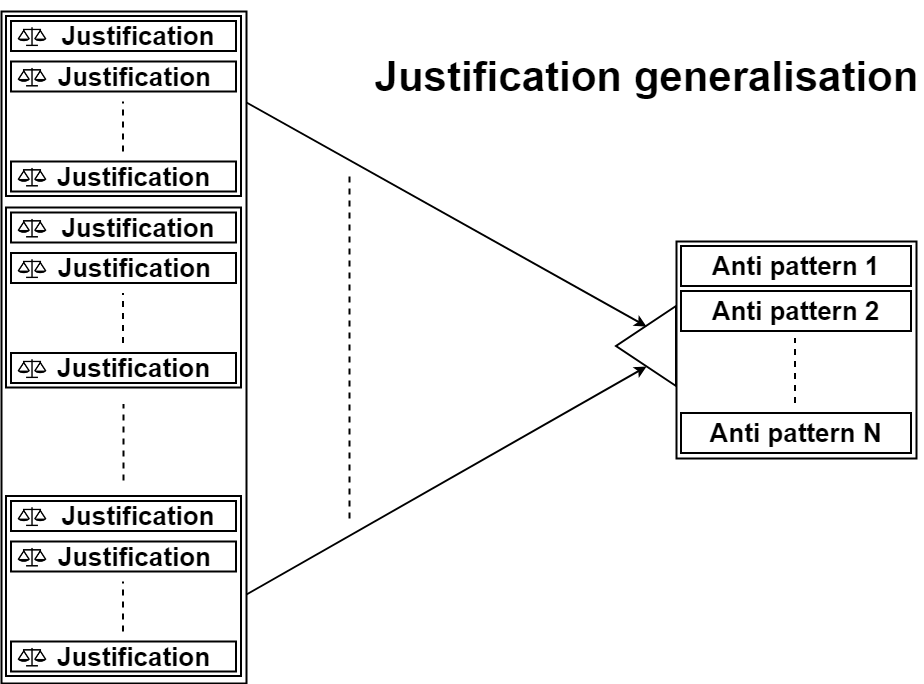
\includegraphics[width=0.45\textwidth]{images/PatternGeneralizing.png}
	}
	\hfill
	\subfloat[A diagram that shows the transformation from Justification to a `anti-pattern'.\label{fig:JustificationtoGeneral}]{%
		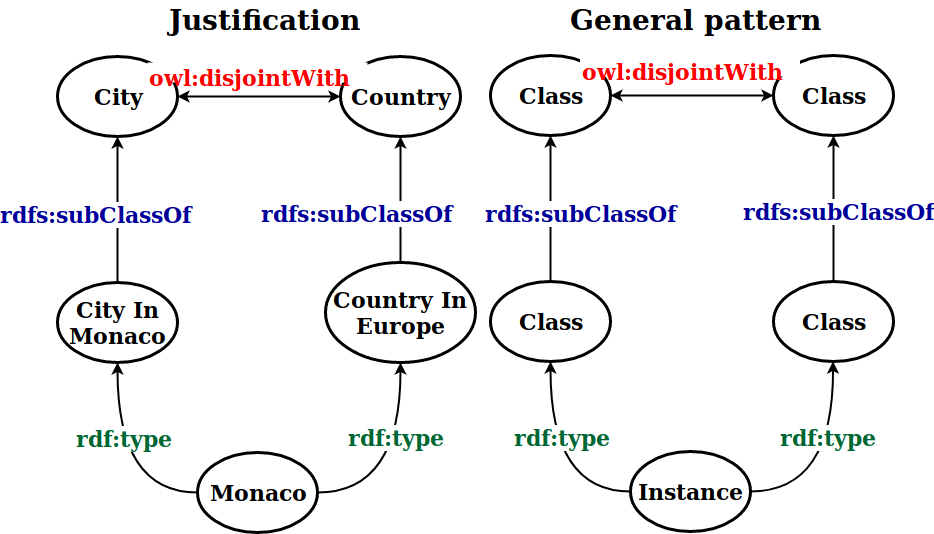
\includegraphics[width=0.45\textwidth]{images/JustificationtoGeneral.png}
	}
	\caption{zoomed in the diagram of the third part of the pipeline, as well as a closer look into justifications and general graphs.}
	\label{fig:PipelinePart3}
\end{figure}
To get the `anti-pattern' from the justification, we first generalise the justification by removing the instantiated subject and object on the nodes as shown in figure \ref{fig:JustificationtoGeneral}. This gives the possibility to generalise the justification purely on its structure instead of its instantiated subject and object. While the information in the nodes is not essential, the information on the edges is. Graphs with different edges can be seen as different contradictions. \\
If we, for example, change the `owl:disjointWith' into `rdfs:subclassOf' and transform one of the `rdfs:subclassOf' into an `owl:disjointWith' We have a different inconsistency pattern. For this reason, we need to store the edges in the `anti-pattern'.\\
With the justifications now devoid of information on the nodes we now group the justifications per `anti-pattern'. This means that each justification that has the same underlying `anti-pattern' is isomorphic, even with respect to the edges in the pattern. \\
To find these isomorphisms we have implemented a version of the VF2 algorithm\cite{LCordella:2004}, with the addition to the algorithm that we also match the edges of the two justifications. Checking if two graphs are not isomorphic is NP-intermediate. Therefore we added in additional heuristics that need to match first before we apply the VF2 algorithm. Firstly we check if a graph has the same number of vertices, the same number of edges, the same amount of degrees, and in our case it also needs to have the same amount of edges based on the edge types we have. If all these matches then we apply the VF2 algorithm to the two `anti-patterns'. If the algorithm matches a justification to the found `anti-patterns', it adds this particular justification to this `anti-patterns', but if no pattern can be matched to the justification, a new `anti-patterns' is formed from this justification. This algorithm continues until all patterns have been matched to their correct `anti-pattern' group.\\

\section{Implementations}
As shown in figure \ref{fig:PipelinePart45} we show the two implementations that make use of `anti-patterns' that we can findwith the previous section. The first implementation is the use case of analysing the knowledge graph in its entirety, as well as looking at how the inconsistencies occur within the larger knowledge graph. We use the analytics of the knowledge graph later in the sampling implementation. Secondly, we showcase that the sampling technique, with respect to the found `anti-patterns' in the graph that we used, produces similar albeit smaller knowledge graphs.

\subsection{Analysing inconsistent knowledge graphs}
In this paper, we show the implementation of analysing knowledge graphs on a range of characteristics. Our analysis of the knowledge graphs is split into two aspects. The first part is the retrieval of general statistics about the knowledge base:
\begin{itemize}
	\item The number of triples of the knowledge graph.
	\item The Expressivity of the logic language that is used in KB.
	\item The number of distinct namespaces in the knowledge graph.
	\item The number of distinct predicates used in the knowledge graph.
	\item The distribution of indegree over all the nodes.
	\item The distribution of outdegree over all the nodes.
	\item The distribution of the Clustering Coefficient over all the nodes in the graph.
\end{itemize}

The second part of the analysis is specifically aimed at inconsistency statistics. We locate all contradictions that match the `anti-patterns' that have been found by retrieving `almost' all `anti-patterns' from the LOD-a-lot. With the `anti-patterns' we can retrieve the needed statistics that characterise the knowledge graph. The metrics that we use in our analysis are:
\begin{itemize}
	\item Amount of `anti-patterns' in the knowledge graph.
	\item Largest `anti-patterns' by a number of basic triple patterns found in the knowledge graph.
	\item Distribution of the occurrences of contradictions found in the knowledge graph.
	\item Distribution of the sizes of `anti-patterns' found in the knowledge graph.
\end{itemize} 

\begin{figure}[!t]
	\subfloat[This diagram shows one of the usecases for the `anti-patterns', namely Analytics.\label{fig:AnalyticsDrawing}]{%
		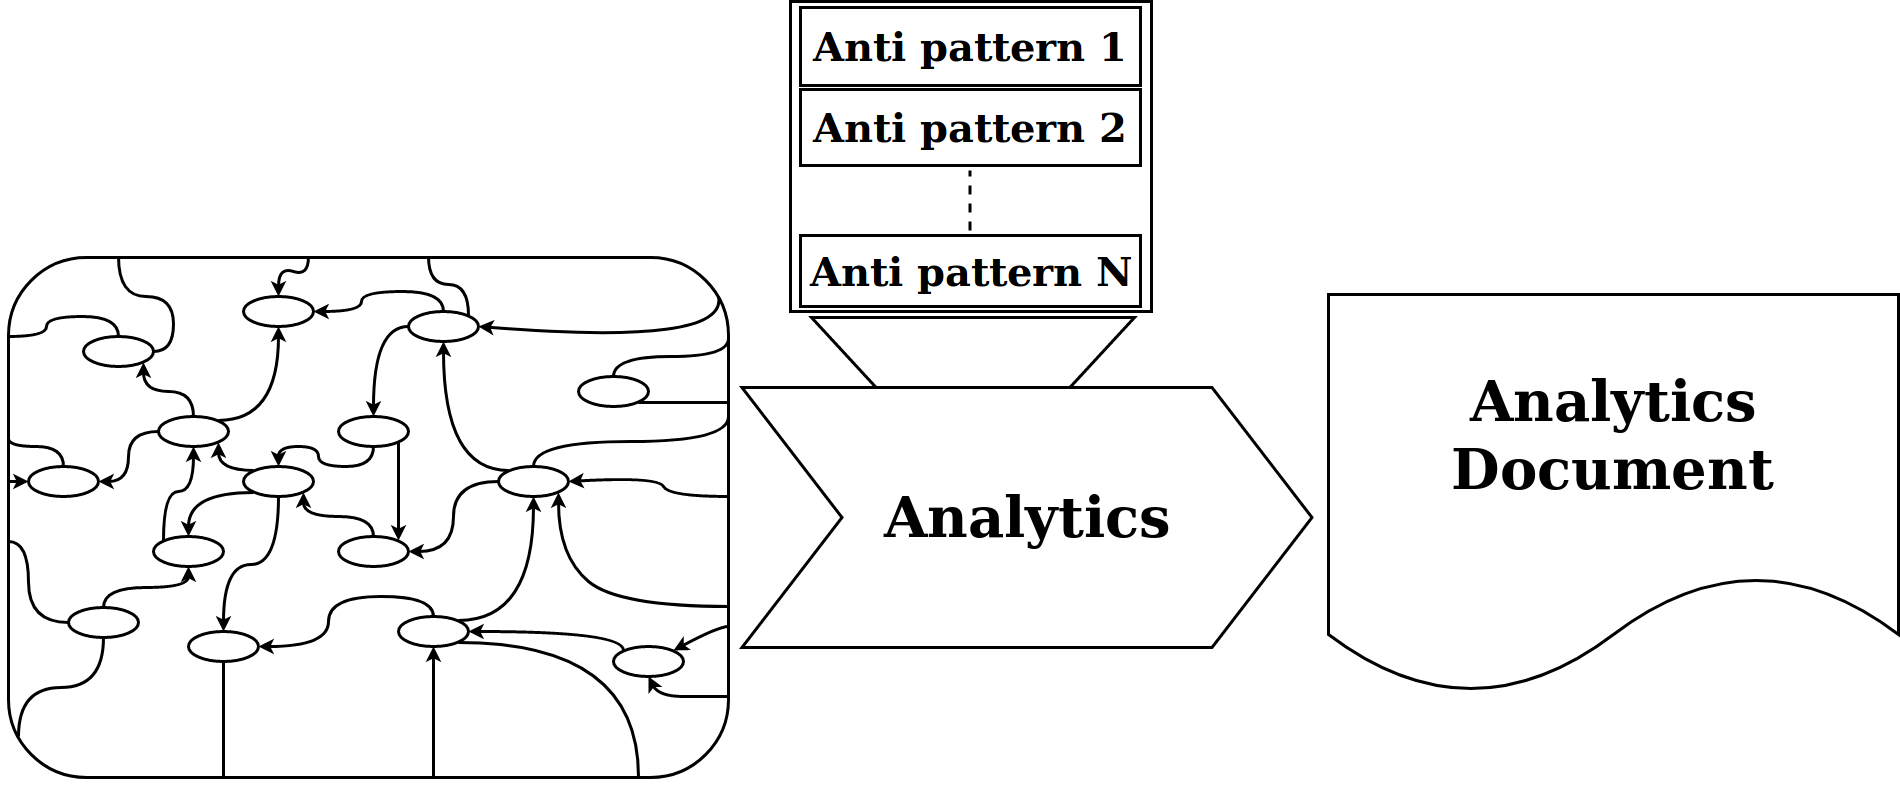
\includegraphics[width=0.45\textwidth]{images/AnalyticsDrawing.png}
	}
	\hfill
	\subfloat[This diagram shows the second usecase for the `anti-patterns', Sampling.\label{fig:SamplingDrawing}]{%
		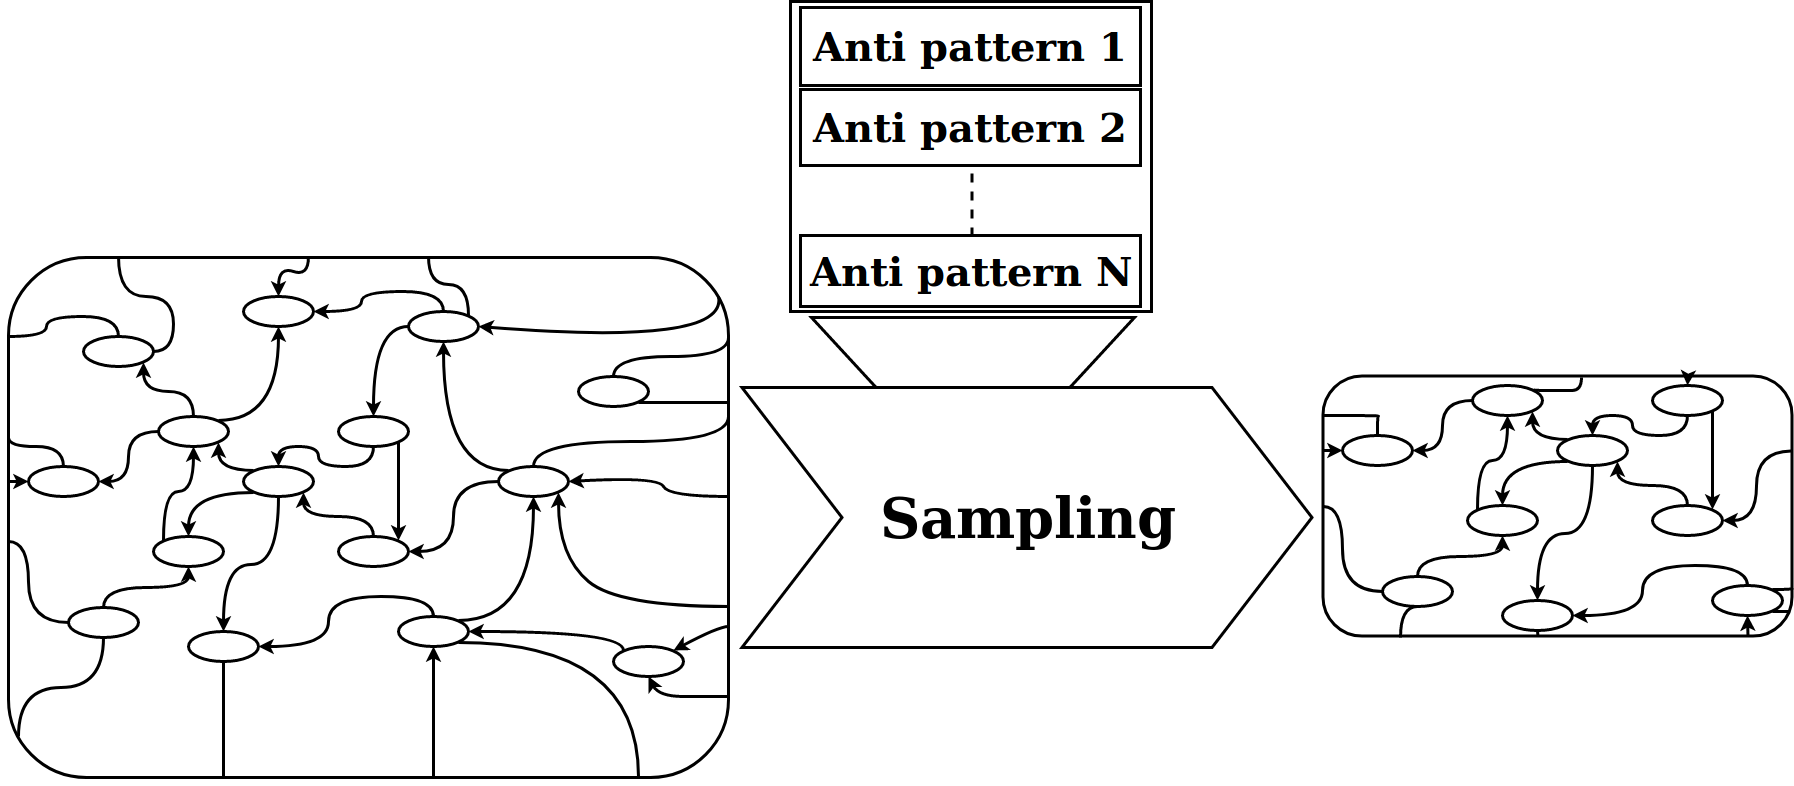
\includegraphics[width=0.45\textwidth]{images/SamplingDrawing.png}
	}
	\caption{zoomed in diagram of the final parts of the pipelines.}
	\label{fig:PipelinePart45}
\end{figure}

\subsection{Sampling inconsistent graphs}
The second implementation that makes use of the `anti-patterns' is the implementation of sampling a knowledge graph. In this paper, the goal of sampling is to sample a knowledge graph into a smaller partition with two constraints. the first constraint is that, we make sure that the knowledge graph stays connected. Secondly, we give the user the possibility to choose the `anti-patterns' and the minimal amount of contradictions that can be in the sample.
To achieve the goal of sampling while keeping the constraints in mind means that we can not use any techniques that start from a node,, or a set of nodes, such as random walks, or forest fire sampling. Because we then cannot guarantee connectedness or the minimal amount of contradictions.\\ 
Our algorithm instead uses random constrained deletion; this algorithm randomly deletes triples that can be safely deleted. Triples that are connected to contradictions, or hold the only connection between subgraphs cannot be deleted.
The first set of triples that can not be deleted are the triples that describe the contradictions. To make sure that contradictions are not deleted, we start by building an HDT\cite{FMPGPA:13}\cite{MPAF:12} that stores all the triples that make up these contradictions. We use a SPARQL query to find the results of each of the `anti-patterns', and retrieve the number of contradictions the user wanted as BTPs. The triples are then combined and converted to an HDT. The algorithm can now check if a triple can be safely deleted. By checking if the triple is not present in the HDT.\\
The second set of triples that can not be deleted are the triples that break the to sample graph into smaller subgraphs. To negate this problem the algorithm uses local connectedness. A triple may only be safely deleted if there is a second path that connects the object and the subject without having to pass through the severed link. There is one exception to the rule when either the subject or the object does not have any other links, the triple is then is also allowed to be deleted. With this, we can guarantee that the graph does not split into smaller subgraphs. \\%TODO: Can we guarantee local connectedness?
The sampling by random deletion now continues to delete triples until the sample reaches the size given by the user, or when it is no longer able to delete triples. This can happen either because the only triples that can be deleted split the graph into subgraphs, or the only triples that can be safely deleted belong to the non-deletable contradictions.


\newpage
\section{Experiments}
\textit{Datasets}. We have implemented the pipeline to retrieve the `anti-patterns' from the LOD-a-lot. We chose the LOD-a-lot, for its size, with 28,362,198,927 triples and the 650,000 different datasets. the `anti-patterns we found form the basis for the analysis and sampling of the test cases, YAGO, Freebase, and DBpedia.\\
We chose these three knowledge graphs, because all three have numerous different characteristics as shown in F\"arber\cite{MichaelF:2017}. With YAGO having over 500.000 classes, and DBpedia having only 736 classes. The number of relations between both YAGO and DBpedia is different, with only 106 relations for YAGO and more than 55,000 relations for DBpedia. With Freebase having both a large number of relations and classes.\\

\textit{Experimental setup}. The implementation was written in Java and is the program has been made available here: >>LINK<<.   % TODO: SERVER SPECS

\subsection{Anti-pattern Analysis}

\subsection{Experiment 1: \textbf{RQ1}:  Can we design a pipeline that can retrieve a (sub-)set inconsistencies and translate the inconsistencies to `anti-patterns'?}
% Describe how the creation of the inconsistencies from the lod cloud worked.
\textit{Experiment description}. The purpose of this experiment is to show that we can indeed extract inconsistencies from an arbitrary knowledge graph, with the pipeline. 
To show that the pipeline works we have tested the algorithm on two extreme cases — the first case being the pizza ontology and the second case the LOD-a-lot.
The pizza knowledge graph is great for measuring the completeness of the inconsistencies found and shows it is measurable if the reasoner can find the different inconsistencies. Which can be easily checked by hand.\\
Because we can not prove that our pipeline guarantees the completeness, we test if the pipeline still retrieves all `anti-patterns' even when the size of the subgraph is 
smaller than the size of the knowledge graph.\\
\textit{analysis}. We compare the results of our method for retrieving the `anti-patterns' from the pizza ontology with the inconsistencies found by the reasoners in prot\'{e}g\'{e}.
The results are summarized in Table \ref{table:GraphStats}. Results of our method show that even with 

\begin{table}[!t]
	\centering
	\makebox[\textwidth]{
		\begin{tabular}{|l|l|l|}
			\hline
			& Inconsistent? & Found inconsistencies \\ \hline \hline
			250 triple subgraphs     & Yes           & 9\\ \hline
			500 triple subgraphs     & Yes           & 9\\ \hline
			1,000 triple subgraphs     & Yes           & 9\\ \hline
			5,000 triple subgraphs     & Yes           & 9\\ \hline
			Pellet                     & Yes           & 6\\ \hline
			HermiT                     & Yes           & 6\\ \hline
			Pellet                     & Yes           & 6\\ \hline
	\end{tabular}}
	\caption{table showing the reasoners to test the pizza ontology.}
	\label{table:PizzaOntology}
\end{table}

\subsection{Experiment 2: \textbf{RQ3}: Implementation 1, Analysing inconsistent graphs}
\textit{Experiment description}. We retrieved the statistics of YAGO, DBpedia knowledge graphs as explained in section 6.  \\

\textit{Analysis}. Table \ref{table:GraphStats} shows the analytics about the knowledge graph. As noticed the results show several distinctions between the three different knowledge graphs. Even though their expressiveness and the size do roughly match their number of namespaces and distinct predicates 
differ between the three test cases.\\

\begin{table}[!t]
	\centering
	\makebox[\textwidth]{
		\begin{tabular}{|l|l|l|l|l|l|l|}
			\hline
			& Size          & Expressivity & Namespaces & Distinct predicates & Amount of `Anti-patterns' &  Largest Inconsistency \\ \hline \hline
			DBpedia & 1,040,358,853 & SHOIN           & 20          & 18                    & 13                         & 19                        \\ \hline    
			YAGO     & 158,991,568  & SHOIN           & 11          & 5                     & 135                        & 19                        \\ \hline
			pizza     & 1,946         & SHOIN           & 29          & 6                     & 2                          & 6                        \\ \hline
	\end{tabular}}
	\caption{table showing several statistics about graphs.}
	\label{table:GraphStats}
\end{table}

\subsection{Experiment 3: \textbf{RQ3}: Use case 2, Sampling inconsistent graphs} 
\textit{Experiment description}. To test the sampling a sample size of 20\% is taken, as the paper by Jure Leskovec and Christos Faloutsos \cite{Leskovec:2006} shows that samples
up to 15\% still hold the characteristics of the original graph well, even with simpler sampling methods. \\

\textit{Analysis}. Table \ref{table:GraphStats} shows the of the analytics about the knowledge graph before the sampling. As noticed the results, shows several distinctions between the three different knowledge graphs. Even though their expressiveness and the size do roughly match their number of namespaces and distinct predicates 
differ between the three test cases.\\
Table \ref{table:GraphStatsSample} shows the analytics of the knowledge graphs after the sampling has been applied. Even though the sample size has been reduced to one-fifth of the original size. The statistics of the sampled knowledge graph still match the original knowledge graph, within the same ballpark scores.
Figures \ref{fig:indegree},  \ref{fig:outdegree},  \ref{fig:Coeff}, show the distribution of statistics of the knowledge graph. %TODO: Expand this.\\
Figures \ref{fig:indegreeSample},  \ref{fig:outdegreeSample},  \ref{fig:CoeffSample} show the distribution of the statistics sampled knowledge graph. As noted, the distribution
of the statistics match the original knowledge graph. \\

\begin{table}[!t]
	\centering
	\makebox[\textwidth]{
		\begin{tabular}{|l|l|l|l|l|l|l|}
			\hline
			& Size          & Expressivity  & Namespaces  & Distinct predicates   & Amount of `Anti-patterns'  &  Largest Inconsistency \\ \hline \hline
			DBpedia     & 1,040,358,853    & SHOIN         & 20          & 18                    & 13                         & 19                        \\ \hline    
			Yago        & 158,991,568     & SHOIN         & 11          & 5                     & 135                        & 19                        \\ \hline
			pizza       & 1,946          & SHOIN         & 29          & 6                     & 2                          & 6                        \\ \hline
	\end{tabular}}
	\caption{table showing several statistics about graphs.}
	\label{table:GraphStatsSample}
\end{table}


\begin{figure}[!t]
	\subfloat[The distribution of indegree over all nodes.\label{fig:indegree}]{%
		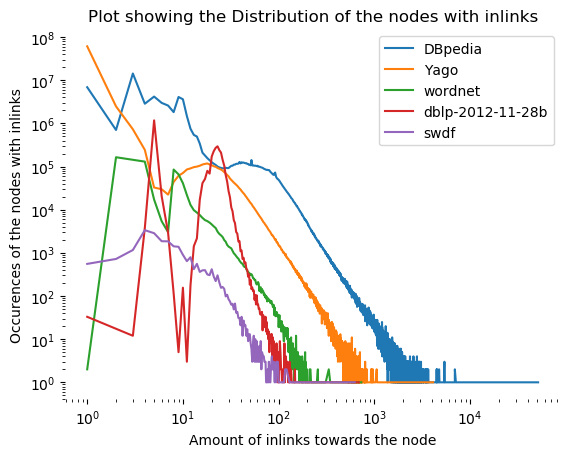
\includegraphics[width=0.33\textwidth]{images/figure4.png}
	}
	\subfloat[The distribution of outdegree over all nodes.\label{fig:outdegree}]{%
		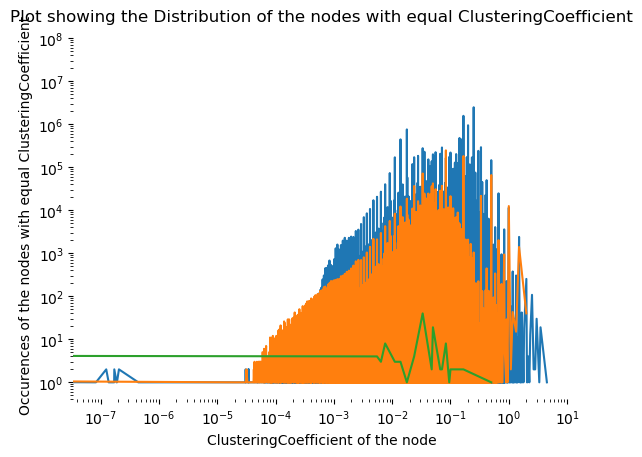
\includegraphics[width=0.33\textwidth]{images/figure5.png}
	}
	\subfloat[The distribution of the Clustering Coefficient over all nodes.\label{fig:Coeff}]{%
		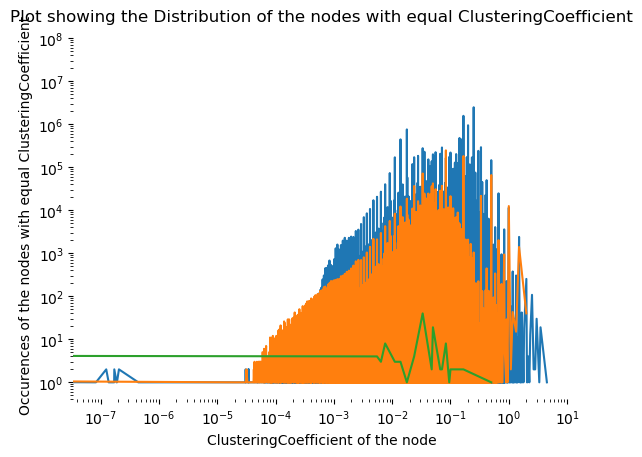
\includegraphics[width=0.33\textwidth]{images/figure5.png}
	}
	\vspace{\floatsep}
	\subfloat[The distribution of indegree over all nodes of the sample.\label{fig:indegreeSample}]{%
		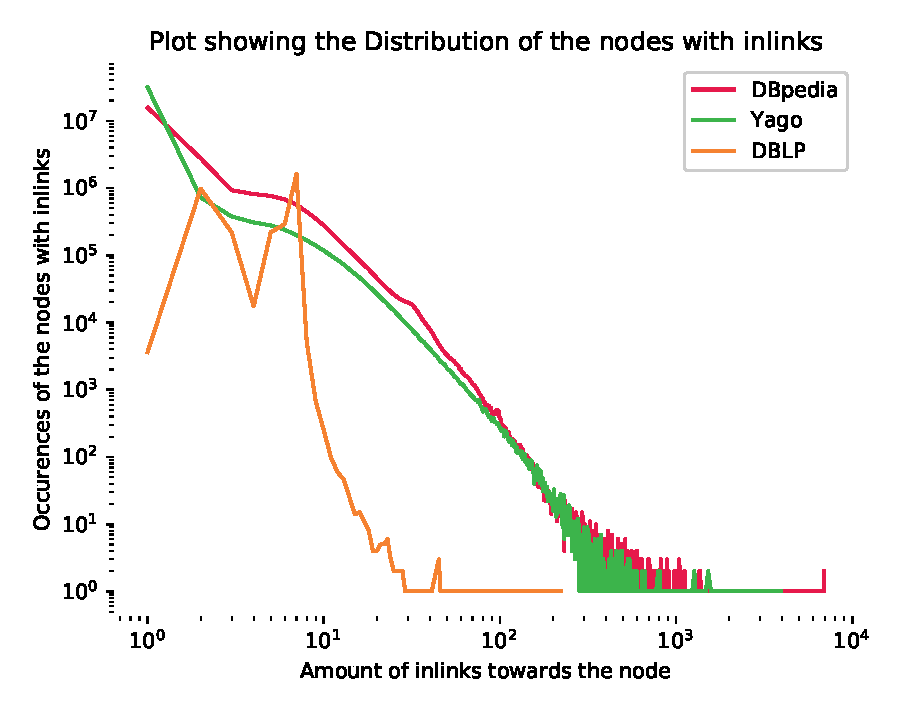
\includegraphics[width=0.33\textwidth]{images/Samplefigure4.eps}
	}
	\subfloat[The distribution of outdegree over all nodes of the sample.\label{fig:outdegreeSample}]{%
		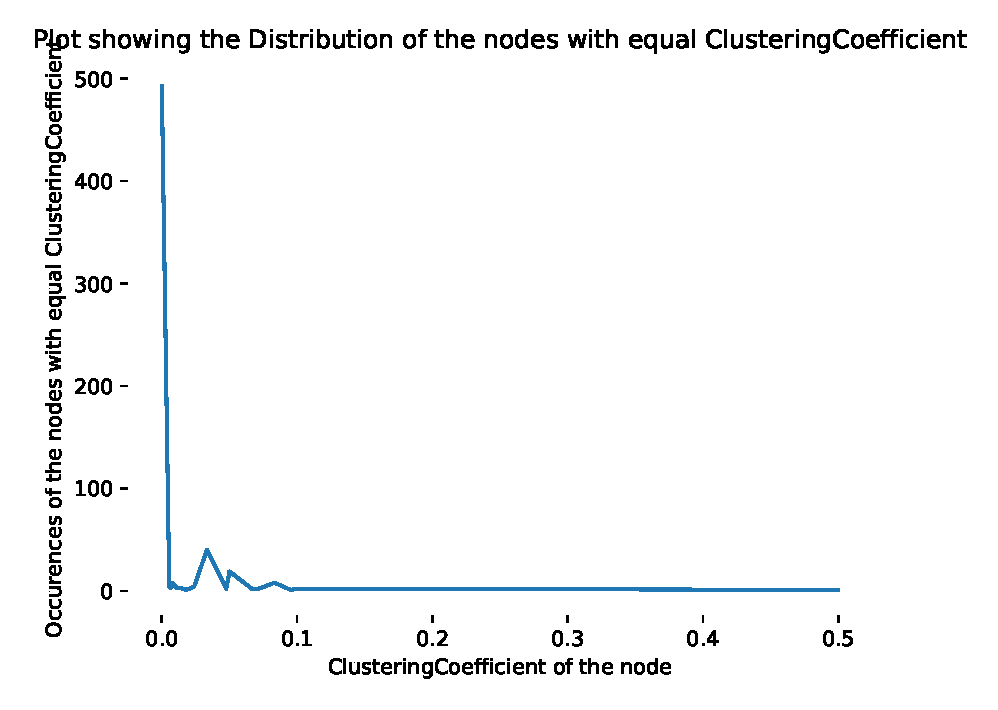
\includegraphics[width=0.33\textwidth]{images/Samplefigure5.eps}
	}
	\subfloat[The distribution of the Clustering Coefficient over all nodes of the sample.\label{fig:CoeffSample}]{%
		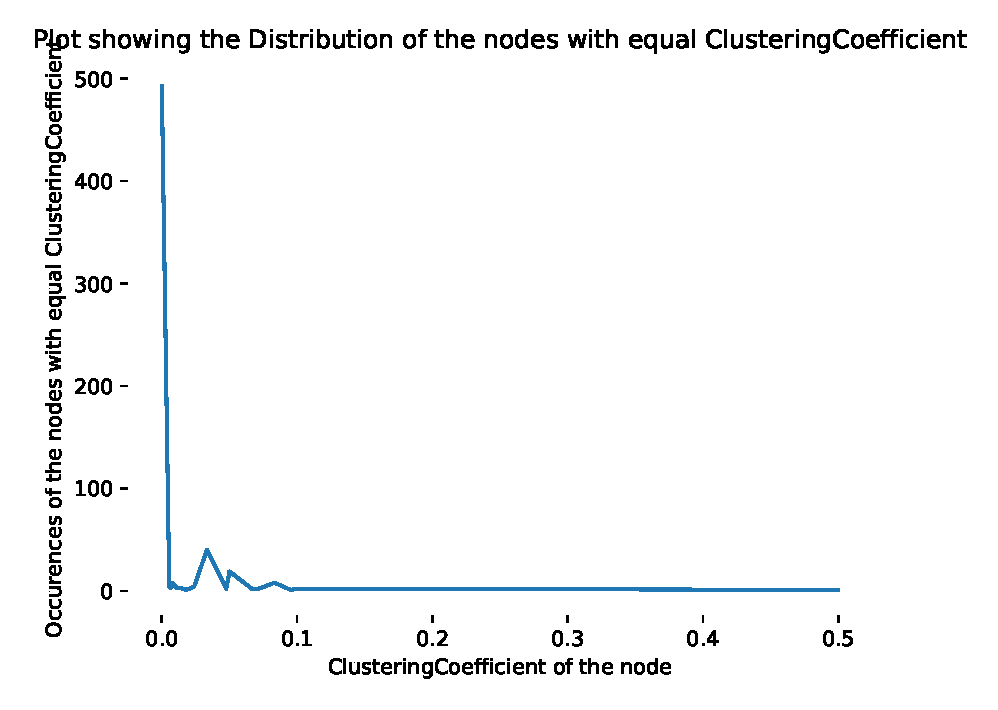
\includegraphics[width=0.33\textwidth]{images/Samplefigure5.eps}
	}
	\caption{Figures showing several statistics about graphs.}
	\label{fig:GraphStats}
\end{figure}


\begin{figure}[ht]
	\centering
	\subfloat[Plot showing the Distribution of size.\label{fig:Size}]{%
		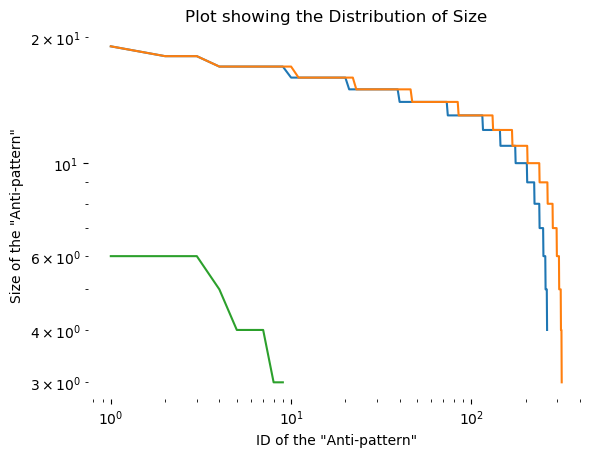
\includegraphics[width=0.33\textwidth]{images/figure1.png}
	}
	\subfloat[Plot showing the Distribution of occurrences.\label{fig:SizeSample}]{%
		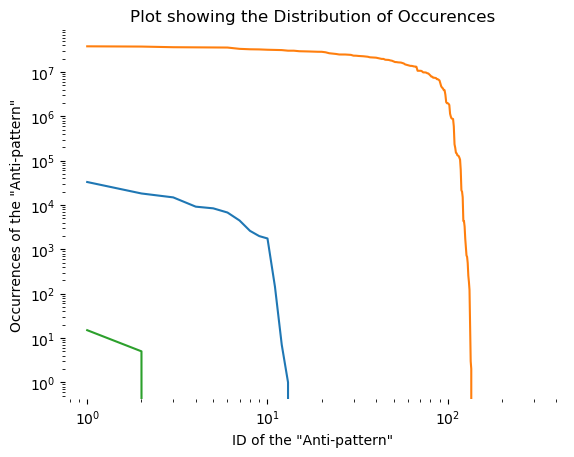
\includegraphics[width=0.33\textwidth]{images/figure2.png}
	}
	\subfloat[Plot showing the Distribution of occurrences.\label{fig:SizeSample2}]{%
		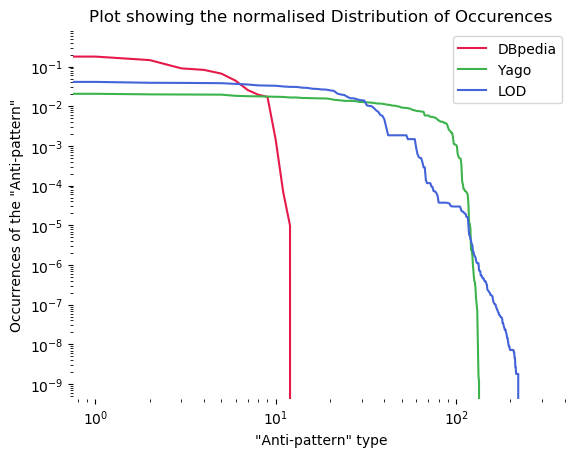
\includegraphics[width=0.33\textwidth]{images/figure3.png}
	}
	\vspace{\floatsep}
	\subfloat[Plot showing the Distribution of size of the Sample.\label{fig:Occurences}]{
		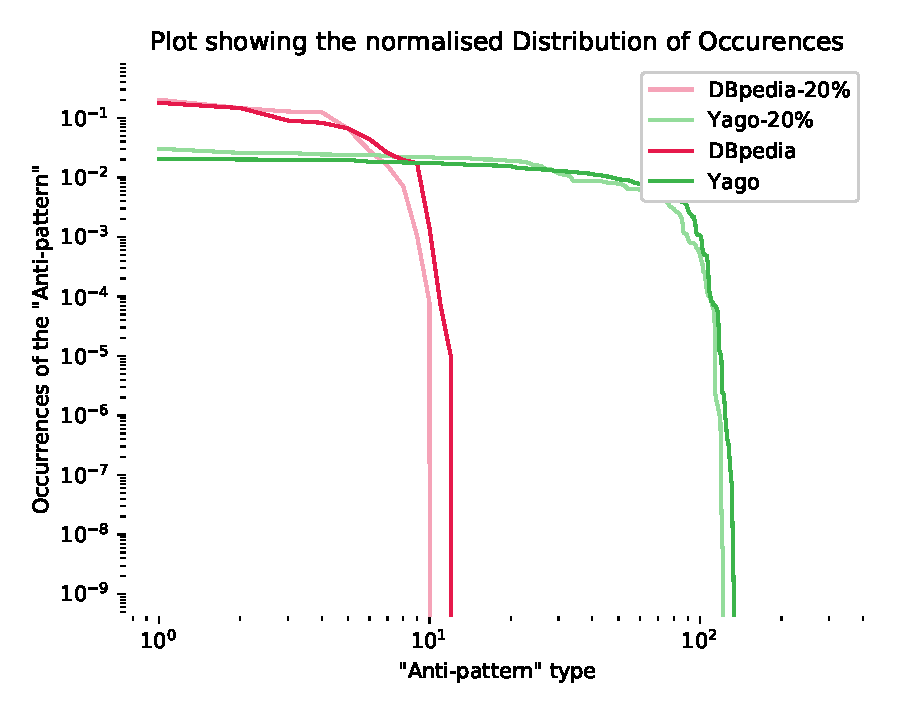
\includegraphics[width=0.33\textwidth]{images/Samplefigure1.eps}
	}
	\subfloat[Plot showing the Distribution of occurrences of Size of the Sample.\label{fig:OccurenceseSample}]{%
		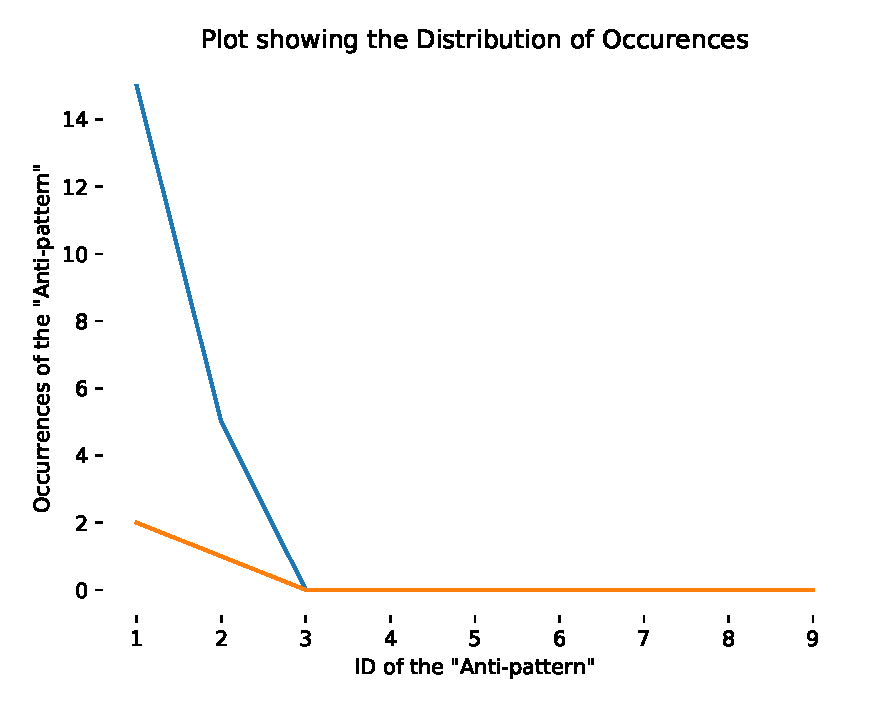
\includegraphics[width=0.33\textwidth]{images/Samplefigure2.eps}
	}
	\subfloat[Plot showing the Distribution of occurrences of Size of the Sample.\label{fig:OccurenceseSample2}]{%
		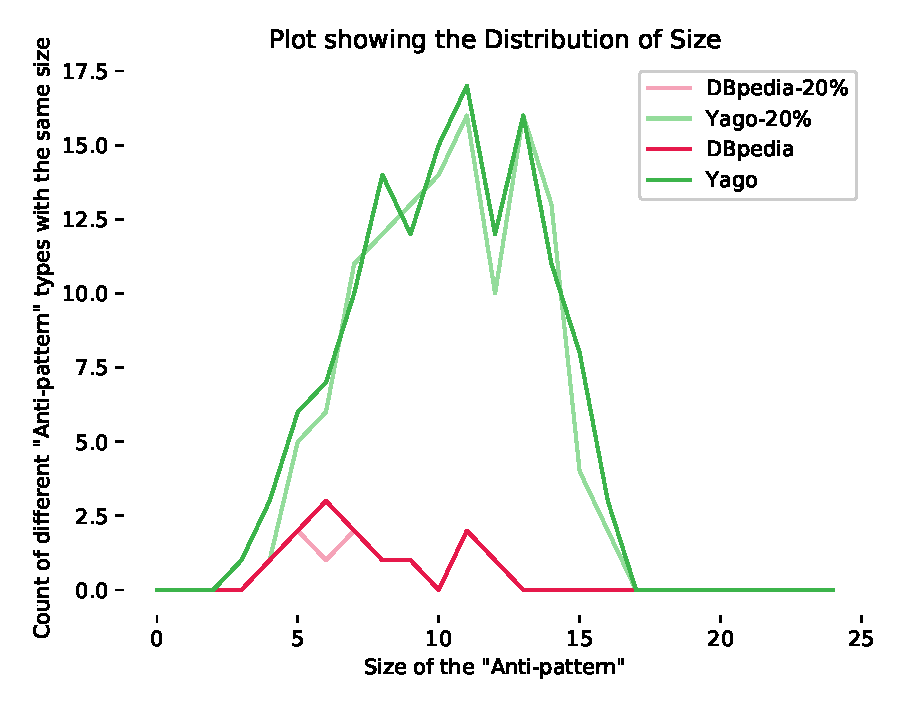
\includegraphics[width=0.33\textwidth]{images/Samplefigure3.eps}
	}
	\caption{Figures showing several statistics about the Anti patterns.}
	\label{fig:Antipattern}
\end{figure}

\newpage
\section{Conclusion}
In this paper, we have created a formal notion for `anti-patterns', patterns describing an error in a knowledge graph that makes the knowledge graph inconsistent. 
We have constructed a pipeline that can extract the `anti-patterns' from any knowledge graph. We then tested the extraction pipeline by extracting `almost' all `anti-patterns' from the LOD-a-lot. \\
We have shown two implementations that make extensive use of the `anti-patterns', knowledge graph analysis and knowledge graph sampling with respect to `anti-patterns'.
With knowledge graph analysis, we can now give qualitative and quantitative information about a knowledge graph with respect to its inconsistency. 
We observed that `anti-patterns' follow the same distribution in each of the large knowledge graphs. the Analysis of the `anti-patterns' also showed that most `anti-patterns' consist out of `rdfs:subclassOf' and `owl:equivalentClass'. `rdfs:range' and `rdfs:domain' do not occur in the `anti-patterns'.
Finally, we showed that knowledge graph sampling with respect to `anti-pattern' is possible. We demonstrate this by sampling knowledge graphs by random deletion.
We show that sampled knowledge graphs still have the same characteristics with original knowledge graphs.\\
\textit{Future Work}. We want to evaluate why `rdfs:range' and `rdfs:domain' do not occur in the `anti-patterns' and we would improve the generalisation of `anti-patterns', by creating more general types for `anti-patterns'. 

\newpage
\bibliographystyle{plain}
\bibliography{ThesisBib}

\newpage
\section{Appendices}
\subsection{Appendix A}

\end{document}


	

